
\documentclass[draft2.tex]{subfiles} 
\begin{document} 

\section{Conclusions} 
\label{sec:conclusions} 

% fig 17 
\begin{figure*} 
\centering 
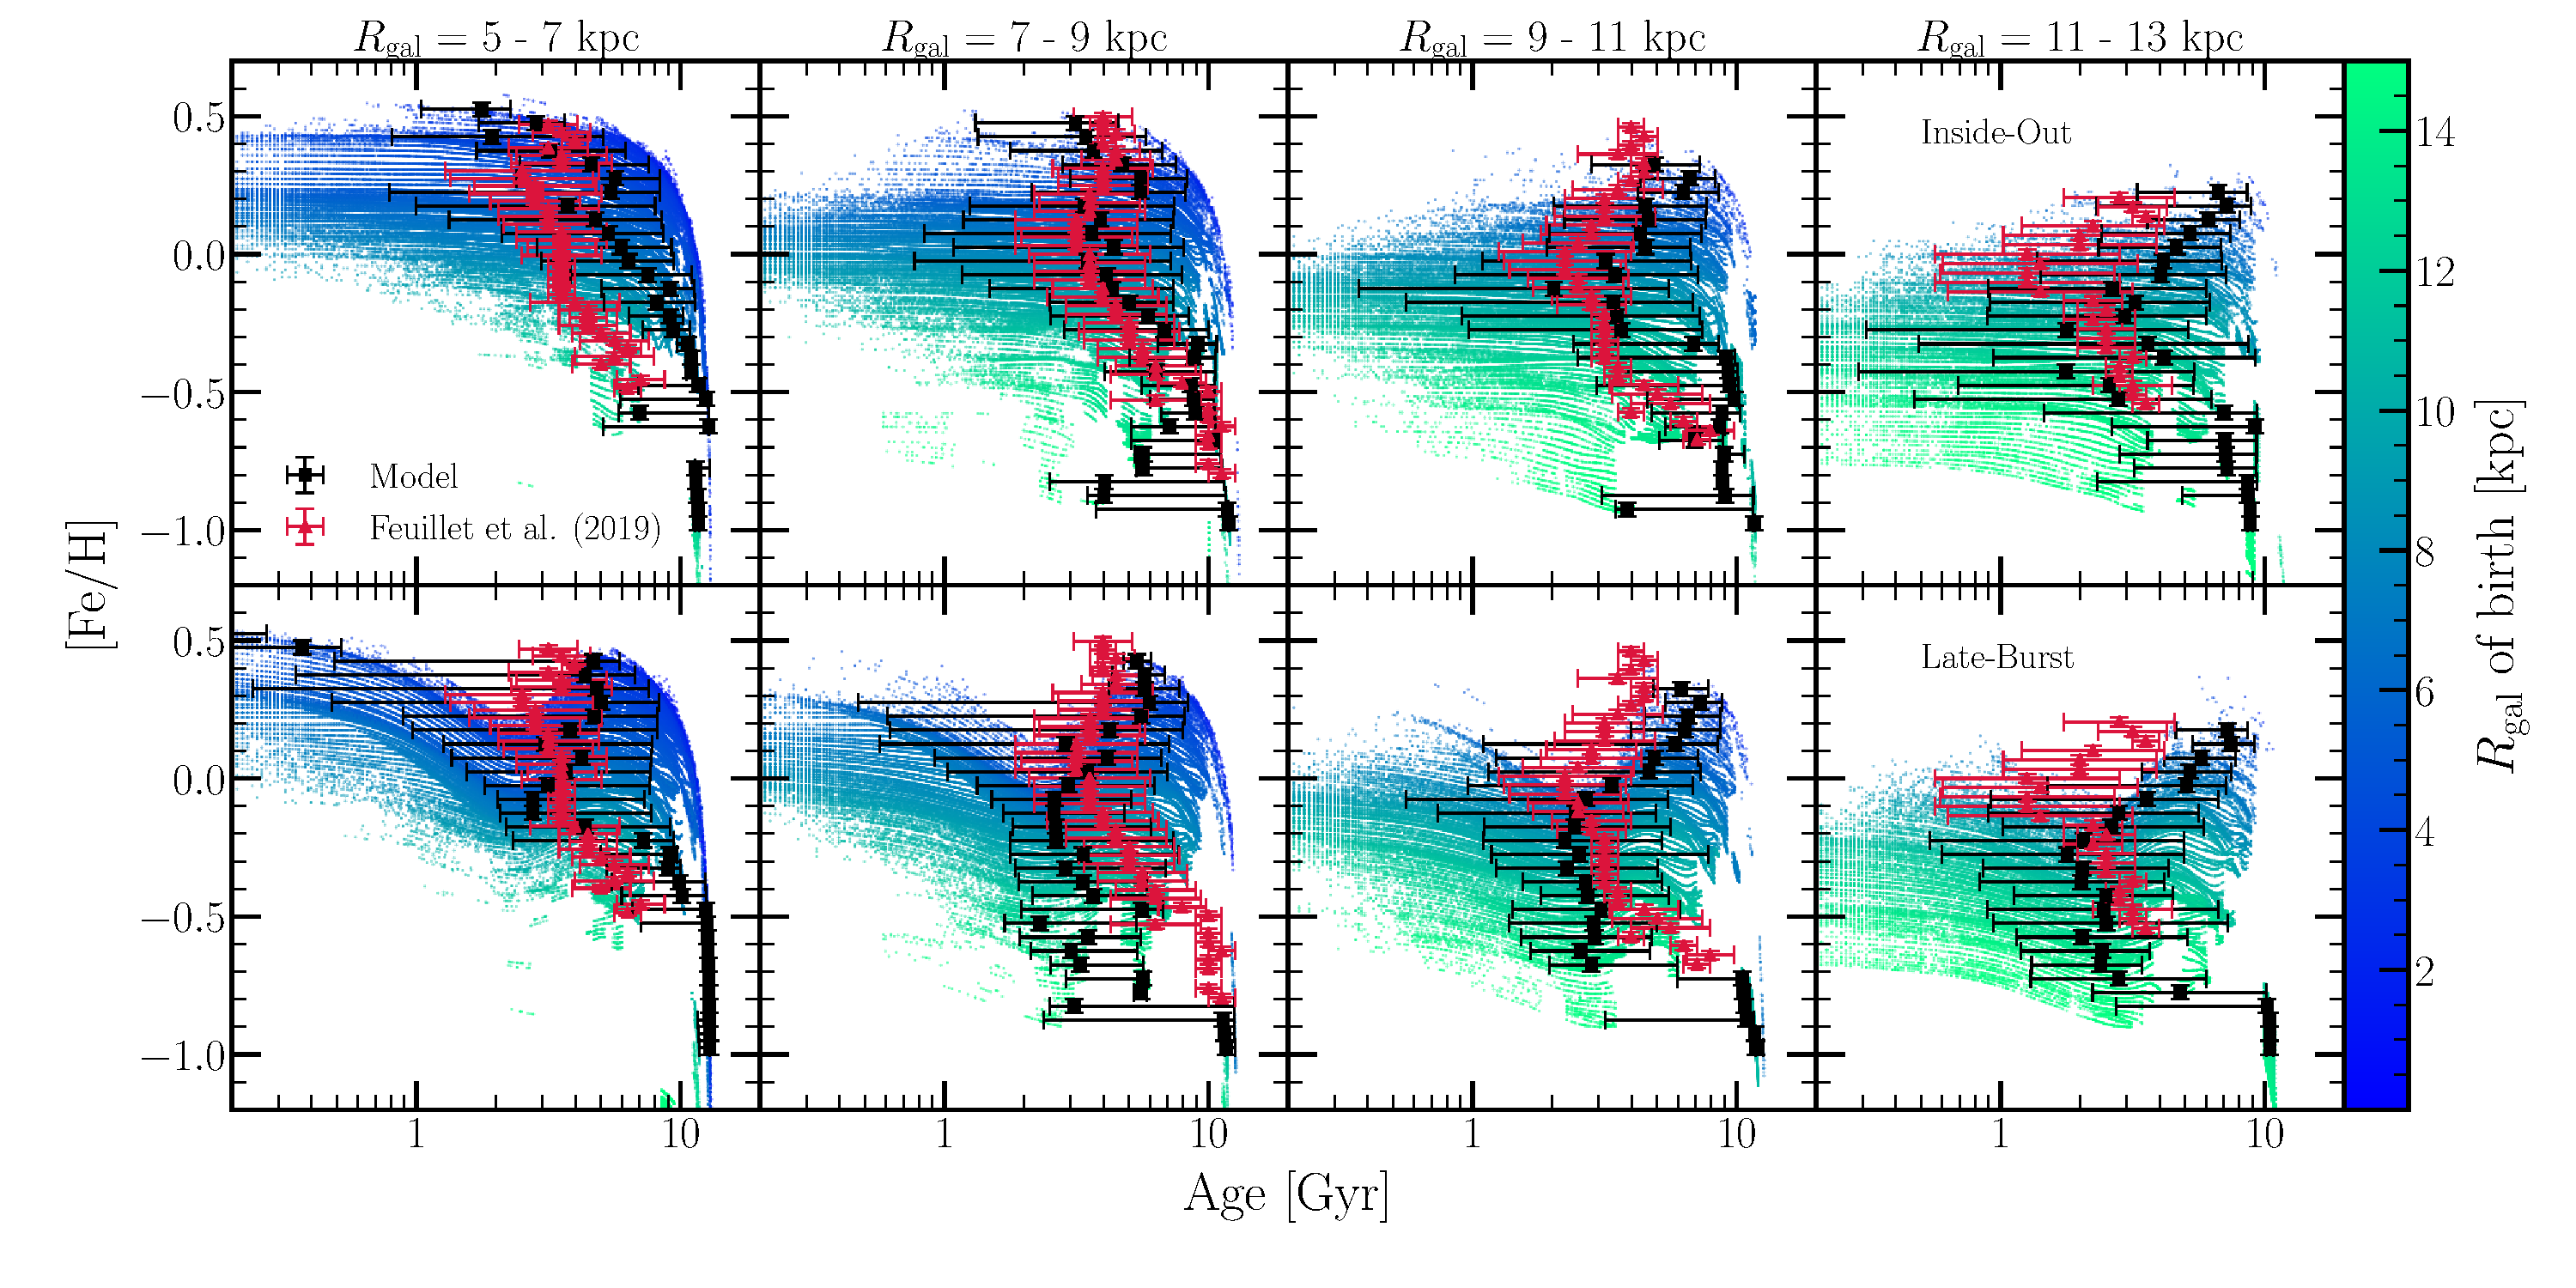
\includegraphics[scale = 0.35]{amr_insideout_vs_lateburst_fe.pdf} 
\caption{The age-[Fe/H] relation predicted by our inside-out (top) and 
late-burst (bottom) SFH models for~$R_\text{gal}$ = 5 - 7 kpc (left), 7 - 9 kpc 
(left middle), 9 - 11 kpc (right middle), and 11 - 13 kpc (right). Each panel 
shows only the~$\left|z\right|\leq$~0.5 kpc population. Red triangles, black 
squares, error bars, and coloured points are as in Fig.~\ref{fig:age_alpha} for 
the corresponding Galactic region, but with the model prediction quantified in 
bins of~$\Delta$[Fe/H] = 0.05. } 
\label{fig:amr_insideout_vs_lateburst_fe} 
\end{figure*} 

In this paper, we have modeled the Milky Way as a series of concentric rings 
with~$\Delta R_\text{gal}$~= 100 pc width, describing each ring as a 
conventional one-zone chemical evolution model and allowing the exchange of 
stellar populations between zones to include the impact of stellar migration in 
the model Galaxy. 
Though there have been other studies that employ a similar methodology 
\citep[e.g.][]{Schoenrich2009a, Schoenrich2009b, Kubryk2015a, Kubryk2015b, 
Sharma2020}, ours and the~\citet{Minchev2013, Minchev2014, Minchev2017} model 
are the only ones that make use of a hydrodynamical simulation to describe 
radial mixing. 
In our case we use the~\hsim~zoom-in simulation of a Milky Way-like disc galaxy 
formed from cosmological initial conditions~\citep{Christensen2012, 
Zolotov2012, Loebman2012, Brooks2014, Bird2020}. 
The simulation provides a prescription for radial migration and vertical 
structure with no free parameters, though there is still a choice to be made 
about how to model the time dependence of migration for a given stellar 
population (see~\S~\ref{sec:methods:migration}). 
In our fiducial prescription, a stellar population traverses the~$\Delta\rgal$ 
between its birth and final radius with a~$\sqrt{t}$ time-dependence 
characteristic of diffusion, as in~\citet{Frankel2018, Frankel2020}. 
While CCSN nucleosynthetic products are deposited instantaneously in the 
population's birth annulus, its SN Ia iron production follows a~$t^{-1.1}$ 
delay-time distribution and is therefore spread across all the annuli that it 
traverses. 
\par 
We adopt supernova yields from oxygen and iron based on a combination of 
theoretical and empirical constraints. 
We base our star formation law on the observed 
$\dot{\Sigma}_\star - \Sigma_\text{g}$ relation in local spirals 
\citep{Bigiel2010, Leroy2013, Krumholz2018a}, with the redshift dependence 
suggested by the observations of~\citet{Tacconi2018}. 
We choose a radially dependent outflow mass loading factor~$\eta(\rgal)$ to 
reproduce observations of the Galactic disc metallicity 
gradient~\citep[e.g.][]{Frinchaboy2013, Hayden2014, Weinberg2019}. 
Our fiducial model adopts an inside-out SFH with e-folding timescales 
calibrated to the~\citet{Sanchez2020} age gradients of low redshift disc 
galaxies (see discussion in~\S~\ref{sec:methods:sfhs}). 
Motivated by the observational results of~\citet{Mor2019} and~\citet{Isern2019}, 
we construct models that exhibit a recent burst in star formation on top of the 
baseline model, as well as a constant SFH model for comparison purposes. 
\par 
We have compared our fiducial inside-out SFH model and its variants to a 
variety of observations, most of them derived from the SDSS APOGEE survey 
\citep{Majewski2017}, finding a number of qualitative successes but also some 
significant qualitative discrepancies. 
\begin{enumerate} 

	\item[\textbf{1.}] The relative number of high-$\alpha$ and low-$\alpha$ 
	stars and the \feh~distribution of these two populations changes 
	systematically with~\rgal~and~\absz, in qualitative agreement with the 
	findings of~\citet{Nidever2014} and~\citet{Hayden2015}. 
	See Fig.~\ref{fig:ofe_feh_diagram}. 

	\item[\textbf{2.}] The~\feh~and~\oh~distributions of stars near the 
	Galactic plane (\absz~$\leq$ 0.5 kpc) change shape, from negatively skewed 
	at small~\rgal~ to roughly symmetric in the solar neighbourhood to 
	positively skewed in the outer Galaxy, in agreement with the findings of 
	\citet{Hayden2015} and with our new measurements based on APOGEE DR16. 
	The influence of radial migration on MDF shape agrees with the simplified 
	model presented by~\citet{Hayden2015} and with the numerical simulation 
	results of~\citet{Loebman2016}. 
	See Figs.~\ref{fig:mdf_3panel_fe} and~\ref{fig:mdf_3panel_o}. 

	\item[\textbf{3.}] Moving up from the midplane, the~\feh~and~\oh~MDFs 
	become more symmetric and less dependent on~\rgal, again in agreement with 
	the observational findings of~\citet{Hayden2015} and the simulation results 
	of~\citet{Loebman2016}. 
	However, the high~\absz~MDFs are not a perfect match to the APOGEE data, 
	especially at~\absz~= 0.5 - 1 kpc where they remain too skewed and too
	\rgal-dependent. 
	See Figs.~\ref{fig:mdf_3panel_fe} and~\ref{fig:mdf_3panel_o}. 

	\item[\textbf{4.}] The distributions of~\ofe~in bins of~\feh~are broad, and 
	their skewness and width change with~\rgal~and~\absz~in qualitative 
	agreement with the APOGEE-based measurements of~\citet{Vincenzo2021a}. 
	However, the model~\ofe~distributions at sub-solar~\feh~do not reproduce 
	the pronounced bimodality found by~\citet{Vincenzo2021a}, and the 
	centroid of the model~\ofe~distribution at super-solar~\feh~shifts upwards 
	with increasing~\absz, a trend not seen in the data. 
	See Fig.~\ref{fig:ofe_mdfs_insideout}. 

	\item[\textbf{5.}] The trend of median stellar age in bins of~\ofe~agrees 
	with the measurements of~\citet{Feuillet2019} in the solar neighbourhood. 
	The width of the log(age) distribution is narrow at high~\ofe~and broad 
	near solar~\ofe, again in agreement with the data. The model predicts a 
	median age-\ofe~relation that is nearly constant over the range 
	\rgal~= 5 - 13 kpc and~\absz~= 0 - 2 kpc, but~\citet{Feuillet2019} find a 
	$\sim$20\% reduction in the median age of high~\ofe~stars at high~\absz. 
	See Figs.~\ref{fig:age_alpha} and~\ref{fig:age_alpha_regions}. 

	\item[\textbf{6.}] While most stars with~\ofe~$\geq$ 0.1 are old, the model 
	predicts a population of young and intermediate-age $\alpha$-rich stars. 
	These stars form in the outer Galaxy (\rgal~> 10 kpc) at times when the SN 
	Ia rate, and thus the iron enrichment, has fluctuated to low values because 
	stellar populations have migrated away before most of their SN Ia have time 
	to explode (see Fig.~\ref{fig:tracks}). 
	This mechanism, which is only realized because we track SN Ia enrichment 
	through rings as populations migrate (\S~\ref{sec:methods:migration}), 
	offers a novel explanation for the existence of young and intermediate-age 
	$\alpha$-rich stars seen in APOGEE~\citep{Chiappini2015, Martig2015, 
	Martig2016, Warfield2021}. 
	See Figs.~\ref{fig:age_alpha} and~\ref{fig:age_alpha_regions}. 

	\item[\textbf{7.}] In the solar neighbourhood, the predicted distribution 
	of stellar age at solar~\feh~or~\oh~is broad, and the trend of median age 
	with metallicity is non-monotonic, with both sub-solar and super-solar 
	metallicity stars being older on average than solar metallicity stars. 
	These predictions agree with the observational results of 
	\citet{Feuillet2019}, though the age scatter is larger than 
	\citet{Feuillet2019} infer, and the agreement of median trends is better 
	for~\oh~than for~\feh. 
	The old population at super-solar metallicity has migrated from the inner 
	Galaxy, as suggested by~\citet{Feuillet2018, Feuillet2019}, and migration 
	produces a non-monotonic age-metallicity relation throughout the disc. 
	The agreement between predicted and observed age-\feh~realtions is 
	noticeably worse at~\rgal~= 5 - 7 kpc and somewhat worse at~\rgal~= 11 - 13 
	kpc. 
	See Figs.~\ref{fig:age_oh_static} -~\ref{fig:amr_insideout_vs_lateburst_fe}. 

	\item[\textbf{8.}] The models with late bursts of star formation, either 
	throughout the disc or at~\rgal~> 6 kpc only (see Fig.~\ref{fig:evol}), 
	achieve better agreement with the~\citet{Feuillet2019} age-\feh~relation 
	over a range of~\rgal. 
	In particular, these models better reproduce the young median ages of solar 
	metallicity stars and the C-shaped form of the observed relation. 
	However, they predict a~$\sim$0.1-dex uptick of~\ofe~at ages of~$\sim$2 Gyr 
	that is not seen in the data. 
	The SFH of these models is empirically motivated~\citep{Mor2019, Isern2019}, 
	and we do not know if there is some variant of our implementation that 
	would preserve their improved agreement with age-\feh~while mitigating 
	their mismatch to age-\ofe. 
	For the other measures listed above, the predictions of these models are 
	qualitatively similar to those of the inside-out model. 
	See Figs.~\ref{fig:age_alpha_regions} and 
	\ref{fig:amr_insideout_vs_lateburst_fe}. 

\end{enumerate} 

All of these predictions are affected by radial migration, and those involving 
vertical trends also inherit the simulation's predicted correlations between 
final~\absz~and the age, birth radius, and final radius of a stellar 
population. 
We regard the overall level of agreement with many distinctive features of the 
Milky Way disc's abundance structure as a significant success of the models. 
However, at least within the framework explored here, it appears that models 
with smooth star formation are not able to explain the pronounced bimodality 
of the observed~\afe~distribution. As discussed by~\citet{Vincenzo2021a}, 
we expect that this problem is generic: a one-zone model with a smooth SFH 
produces an~\afe~distribution that peaks at low values, so it is difficult 
to create a superposition of such models that has a bimodal distribution. 
\par 
The most widely explored solution to this problem involves a two-phase SFH, 
with gas accretion resetting the ISM to low metallicity in between the two 
epochs. 
Versions of this scenario arise in two-infall GCE models 
\citep[e.g.][]{Chiappini1997, Spitoni2019a, Khoperskov2021} and in cosmological 
simulations that give rise to bimodal~\afe~\citep{Mackereth2017, Grand2018, 
Buck2020b}. 
An alternative scenario proposed by~\citet{Clarke2019}, motivated by 
hydrodynamic simulations, attributes the low-$\alpha$ sequence to an 
evolutionary track with low star formation efficiency and the high-$\alpha$ 
sequence to clumpy bursts of star formation that self-enrich with $\alpha$ 
elements. 
In a third, possibly fanciful scenario proposed by~\citet{Weinberg2017}, 
increased outflow efficiency at late times causes the low-$\alpha$ population 
to evolve ``backwards'' to lower~\feh, after formation of the high-$\alpha$ 
sequence. 
Radial migration is likely to reshape the predictions of any of these scenarios, 
even if it does not fully explain bimodality on its own. 
These scenarios can be easily realized within our modeling framework by 
changing the SFH, star formation efficiency, and outflow parameterizations. 
We intend to explore them in future work, seeking observable signatures that 
can distinguish these alternative explanations for one of the most striking 
features of the disc abundance distribution. 
\par 
The computational speed of our hybrid chemical evolution methodology makes it a 
valuable complement to calculating chemical evolution within full hydrodynamic 
cosmological simulations~\citep[e.g.][]{Mackereth2017, Grand2018, Naiman2018, 
Buck2020b, Vincenzo2020}. 
For a given cosmological simulation, we can consider many different choices of 
yields and chemical evolution parameters, varying them individually to isolate 
physical effects and exploring parameter space to identify good fits, 
degeneracies, and persistent discrepancies with data. 
There are many obvious directions to go in extending this approach. 
One is to apply it to additional cosmological simulations to understand the 
impact of different dynamical histories, and to add the ability to model 
stellar populations accreted from satellites. 
A second is to consider additional elements that probe different 
nucleosynthetic pathways; many of these are already incorporated in~\vice, and 
it is easy to add other elements and sources to models. 
A third is to include treatment of radial gas flows and fountains, both of 
which have been explored in more idealized GCE models (e.g.,~\citealp{Lacey1985, 
Bilitewski2012, Kubryk2015a, Kubryk2015b};~\citealp*{Spitoni2013}; 
\citealp{Pezzulli2016, Sharda2021a, Sharda2021b}). 
More ambitious is to implement treatment of stochastic enrichment and 
incomplete ISM mixing~\citep[e.g.][]{Montes2016, Krumholz2018b, Beniamini2020}, 
which have so far been little explored in the context of Milky Way disc 
evolution but which are likely important in understanding the detailed 
correlations of elemenal abundances~\citep{Ting2021}. 
As multi-element spectroscopic surveys grow even faster in scope and precision, 
efficient and flexible theoretical models will be essential for extracting the 
lessons they have to teach about the origin of elements and the history of the 
Milky Way. 

\end{document} 
